% ==================================================================================================================
\section{Rotterdam: Revenue Management in Public Transportation with Smart-Card Data Enabled Agent-Based Simulations \textsuperscript{\footnotesize{\footnote{This research was supported by Netherlands Organisation for Scientific Research (NWO)
Complexity Grant No. 645.000.001 awarded to Dr. Ting Li and Prof.mr.dr. Peter Vervest from
Rotterdam School of Management. It was presented at MATSim User Meetings in 2011 and 2012,
INFORMS International 2012 Beijing, the 7th Workshop on Agents in Traffic and Transportation at
AAMAS 2012 Valencia, Erasmus University Rotterdam, Berlin Institute of Technology, Tsinghua
University and Beijing Jiaotong University.}}}}
\label{sec:rotterdam}
\hfill \textbf{Authors:} Paul Bouman, Milan Lovric

% ==================================================================================================================
In \citet[][]{LovricEtAl_DSS_2013} and \citet[][]{BoumanEtAl_AAMAS_2012} we proposed two scenarios for studying revenue management in public transportation via time-based pricing strategies, such as peak markups and off-peak discounts, nowadays being used by various transit agencies. To evaluate this approach, we developed agent-based simulations using the simulation toolkit MATSim and a transportation demand generated from smart-card data collected in a Dutch urban area. In the first scenario, we simulated only a metro network, while in the second scenario we considered a multi-modal network consisting of metro, tram and bus.

In \citet[][]{LovricEtAl_DSS_2013} we designed and implemented a decision support system for sustainable revenue management that can evaluate the impact of various revenue management strategies on economic, social, and environmental performance. Figure~\ref{fig:rotterdam} shows the structure of the decision support system built on top of the MATSim framework. Smart card transactions (individual check-in and check-out transactions made at stations' entrance and exit gates) were used to reconstruct daily tours of individual passengers. These were inputted into the MATSim simulator as the initial demand. Furthermore, information about the transit network and vehicle schedule was extracted from the OpenStreetMap data and the public transit operator's web site, respectively. Revenue management experiments were then conducted by applying various time-based pricing strategies defined as percentage-wise discounts or markups (applied on top of the nominal price) during specific periods of the day. 

MATSim's core cycle consisting of the mobility simulation, scoring function and replanning was adapted for studying time-based pricing. Firstly, an event handler was created to calculate travel fare of the whole daily tour for each individual (this was implemented according to the real-life pricing scheme: a fixed fee applied at check-in plus a variable distance-based fee applied at check-out). Secondly, we adapted the original Charypar and Nagel scoring function \citep[][]{CharyparNagel_Transportation_2005} by adding the disutility of the travel fare. The existing MATSim's time mutator was used as a replanning strategy to allow passengers to discover more affordable travel times when pricing strategies were enforced (however, a trade-off was introduced by applying a penalty for arriving outside of the expected arrival window that was based on the check-out times observed in the smart card data).

To capture the impact of revenue management on the three sustainability dimensions, we added event handlers to produce a number of relevant key performance indicators (KPIs). The economic performance was measured by the public transit operator's (PTO) revenue, passenger kilometers and vehicle load factors. The social performance was measured by the availability of seating places (as a proxy for passenger comfort) calculated from vehicles loadings after the mobility simulation. We also looked at the average tour price as the measure of public transportation affordability. The impact of a pricing policy on the environment was expressed as the change in carbon footprint stemming from a possible shift of demand between public transportation and private cars (calculated from the change in average tour price and the elasticity of demand). 

Our results show that, by using a smart-card enabled decision support system and by taking a customer-centric view, PTOs can better explore the space of feasible solutions in a broader policy-making context that includes all three dimensions of people-profit-planet sustainability. We validated our approach by comparing the simulation-generated travel fares in the nominal scenario with actual fares recorded in the smart card transactional database \citep[see][]{LovricEtAl_DSS_2013}.

To further study the opportunities of smart card data for demand generation, in paper by \citet[][]{BoumanEtAl_AAMAS_2012} we introduced a pattern-based demand generation method using smart card transactions of three different modalities (metro, tram and bus) in an urban area of The Netherlands as an input. In addition to the use of observations for a single day to generate activity-based demand, daily commuting patterns detected from longitudinal observations for a single smart card were generated. In the specific study, the generated demands were utilized to analyze time-shifting behavior under two different revenue management policies: a plain tariff (with a fixed price per journey and a price per unit of traveled distance) and an off-peak discount. The experiment was repeated for different amounts of pattern-based demand, where the varied parameter was the number of observed samples required for a smart card to be included. 

In the generated demand, the agents which were not generated using pattern-based demand had to replicate their observed tour or trip within 15 minute windows of the observed arrival and departure times. The pattern-based agents had time windows dependent on the observed standard deviations in passengers' actual commuting travel patterns, which were used as a proxy for their time flexibility. This aspect of the demand modeling was more detailed than in study of \citet[][]{LovricEtAl_DSS_2013}, in which agents were assumed homogeneous with respect to their time flexibility. This flexibility was exploited by the time shift mutator which was made available in MATSim as one of the replanning strategies. In future work, improvements in the scoring function and the use of more sophisticated pattern-based demand generation approach need to be considered in order to create more realistic scenarios for a study of time-shifting behavior under revenue management policies.

\createfigure%
{Rotterdam scenario: Decision support system for sustainable revenue management in public transportation}%
{Rotterdam scenario: Decision support system for sustainable revenue management in public transportation}%
{\label{fig:rotterdam}}%
{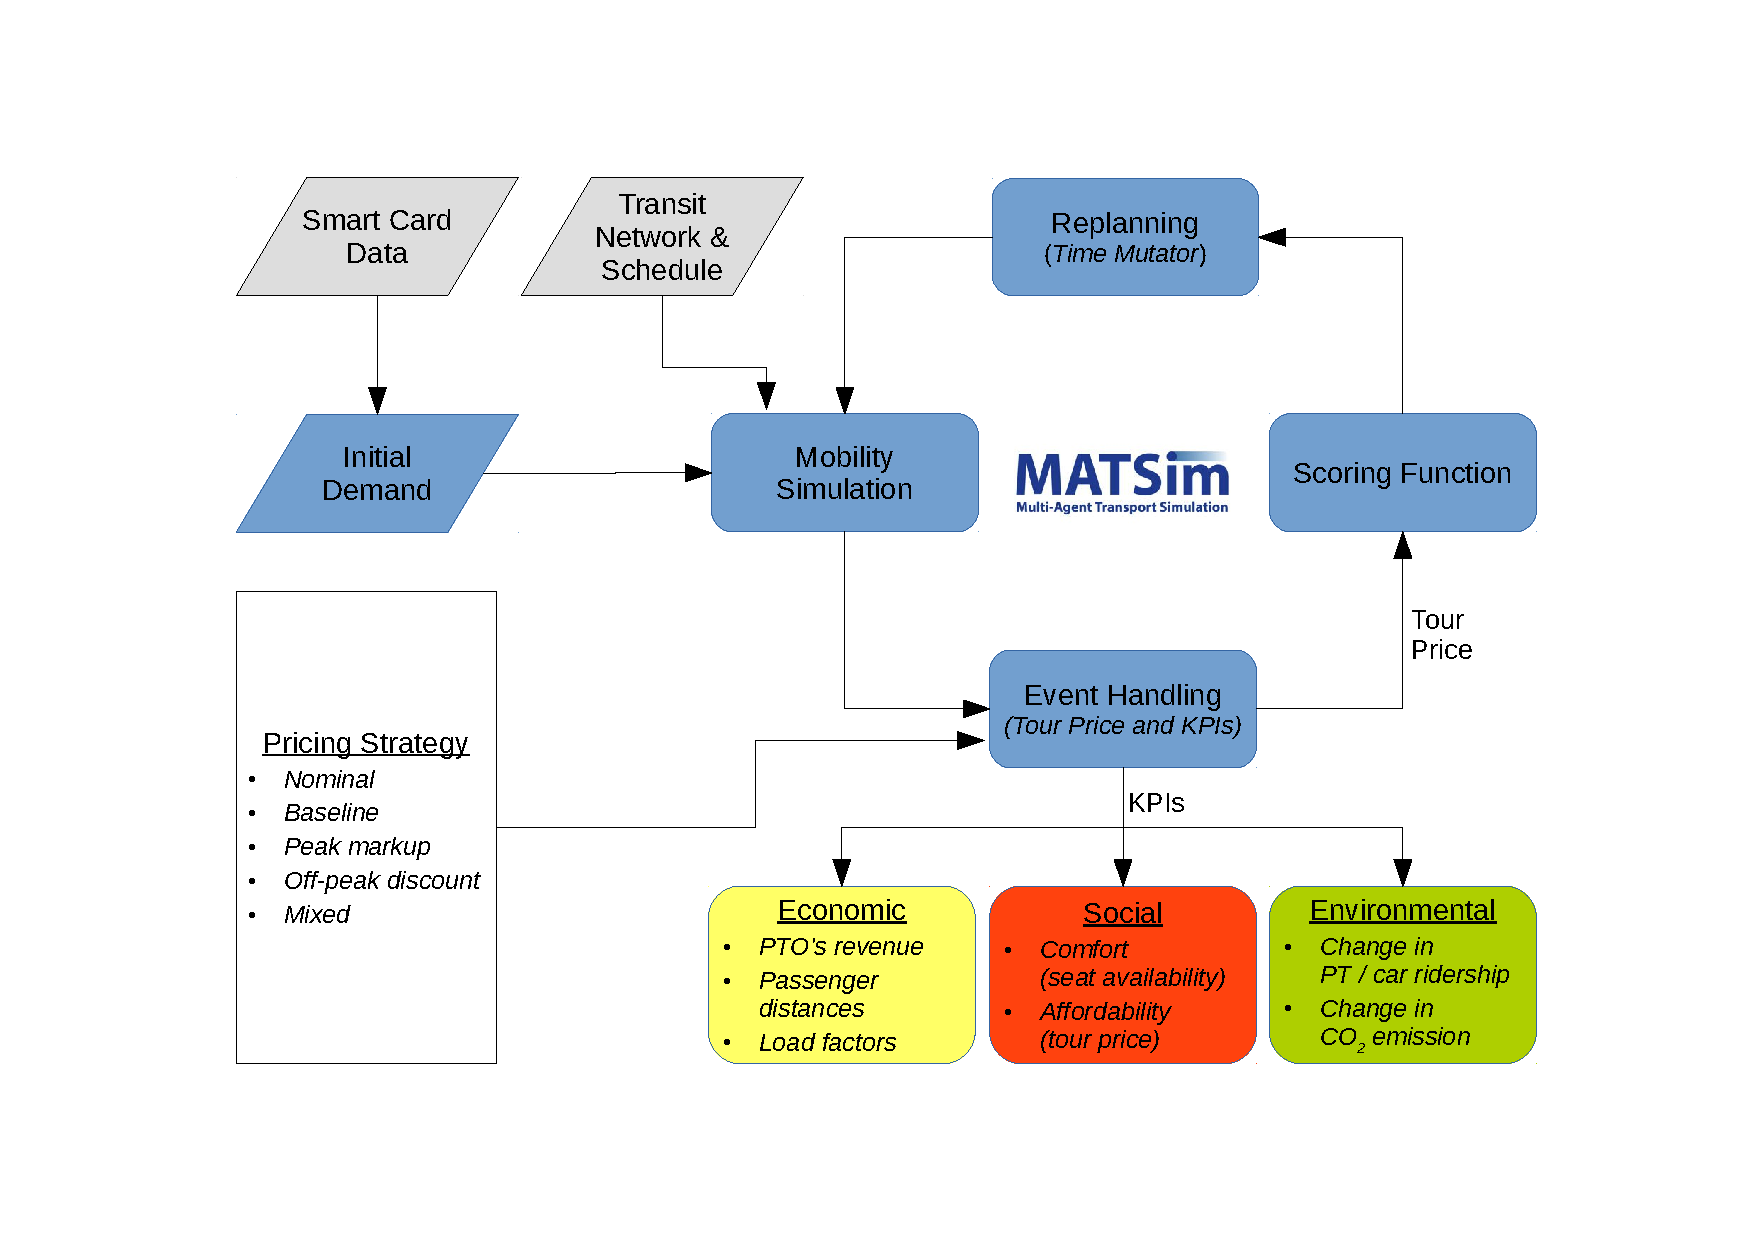
\includegraphics[width=0.85\textwidth, angle=0]{./using/figures/rotterdam}}%
{}

% ==================================================================================================================

